\documentclass[11pt, letterpaper]{article}
\usepackage[margin=0.5in]{geometry}
\usepackage{graphicx}

\begin{document}

\title{Search and Retrieval Algorithms}
\author{Ryan Layer}
\maketitle

\section{Introduction}

Searching for a value in a list is a fundamental operation that many
algorithms can solve, each with unique performance characteristics.  These
distinct features determine the suitability of each algorithm for specific
problem types.  Here, we explore the empirical time and memory tradeoffs of
three popular options: binary search, merge search, and hash table search.
Binary search sorts the database and then uses binary search to find each
query in the database ($O(D \log D) + O(Q \log D)$). Merge search sorts both
lists and then uses the merge operation to step through the lists in order to
find matches ($O(D \log D) + O(Q \log Q) + O(Q + D)$). The hash table search
places each database element in the database into a hash table and then looks
for each query ($O(D) + O(Q)$, amortized). As expected, hash tables were the
fastest and used the most memory, making them ideal for scenarios where
database size is not a constraint. Notably, merge search outperformed binary
search in handling large query sets, and should be used when the query set
constitutes at least 50\% of the database size.

\section{Results}

As expected, the hash table search was between 2X and 5X faster than the
other methods but required over 4X more memory~(Figure \ref{fig:timeandmem}).
Binary and merge search had identical memory footprints and similar runtime
across the query set size range, with binary search slightly faster than
merge search for small query sets and merge search slightly faster for larger
query sets. Theoretically, we did not expect merge search to be faster than
binary search~(Figure \ref{fig:timesim}).
%%%% Add your experiment here %%%%
Memory usage was flat for all methods, indicating that the constant database
size was the most significant factor.

\begin{figure}[ht] \centering
    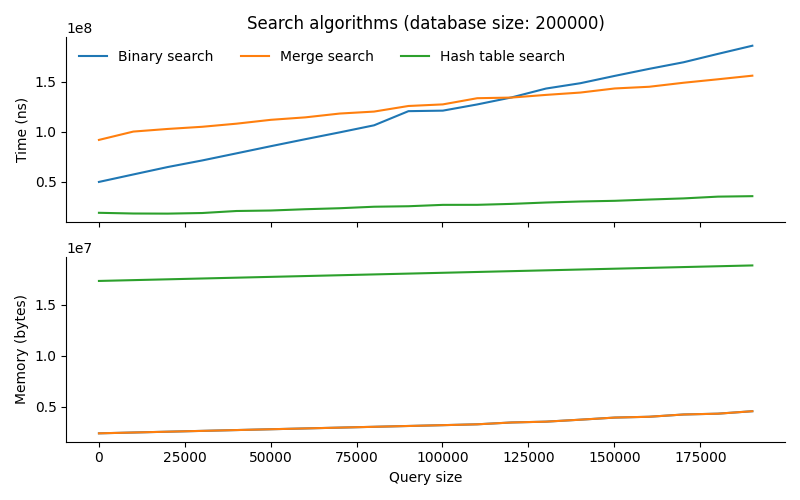
\includegraphics[width=0.6\textwidth]{q100-10000_d200000_str}
    \caption{The empirical runtime and memory usage of search algorithm
    considering a database with 200,000 strings and a varying number of
    string queries.}
    \label{fig:timeandmem}
\end{figure}

\begin{figure}[ht]
    \centering
    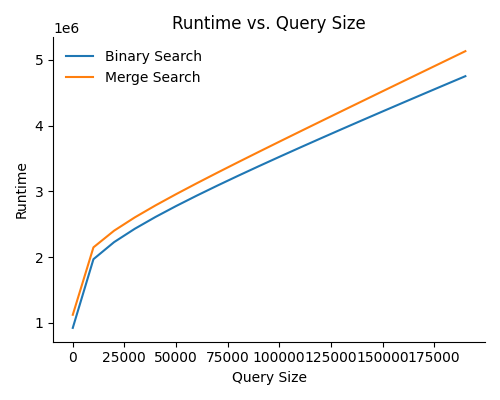
\includegraphics[width=0.5\textwidth]{q100-10000_d200000_sim}
    \caption{The theoretic runtime and memory usage of binary search 
    ($O(D \log D) + O(Q \log D)$) and merge search 
    ($O(D \log D) + O(Q \log Q) + O(Q + D)$) algorithms considering a
    database with 200,000 strings and a varying number of string queries.}
    \label{fig:timesim}
\end{figure}

%%%% Add your figure here %%%%

\section{Methods}

\subsection{Empirical comparison}

We measured the time and memory usage of binary, merge, and
hash table searches considering a database of 200,000 strings and query sets
ranging from 100 to 200,000 strings. Strings for the database and query sets
were drawn randomly from a word list without replacement. We created a new database and query set for each query set size and ran each search method, recording the run time and memory usage separately. We repeated this step five times and retained the meantime and memory metrics.

\subsection{Theoretical comparison}

To compare the theoretical performance of binary search and merge search,
we used $\mathcal{T}(D,Q)=O(D \log D) + O(Q \log D)$ as the theoretical
runtime function for for binary search and $\mathcal{T}(D,Q)=O(D \log D) +
O(Q \log Q) + O(Q + D)$ as the theoretical runtime for merge search, where
$D$ is the database size and $Q$ is the query set size. We then set $D=200,000$, let $Q$ vary from 100 to 200,000, and plotted the runtime.

%%%% Add your method here %%%%

\subsection{Reproducibility}

To replicate these experiments, clone the repository and then run the
empirical and simulation experiments as follows:
\begin{verbatim}
$ clone https://github.com/ryanlayerlab/search.git
$ cd search
$ python src/search.py \
    --query_range 100 200000 10000 \
    --database_size 200000  \
    --rounds 5 \
    --values_file data/words.txt.gz \
    --out_file doc/q100-10000_d200000_str.png
$ python sim.py \
    --query_range 100 200000 10000 \
    --database_size 200000  \
    --width 5 \
    --height 4 \
    --out_file ../doc/q100-10000_d200000_sim.png 
\end{verbatim}
%%%% Add your command here%%%%

\end{document}
